\documentclass[a4paper,10pt]{IEEEtran}
\usepackage{mathptmx}

\usepackage{tabularx} % extra features for tabular environment
\usepackage{amsmath}  % improve math presentation
\usepackage{float}
% \usepackage{pdfpages}

\usepackage{subfig}

\usepackage{graphicx} % takes care of graphics including machinery
\graphicspath{ {./figures/} }
%\usepackage[margin=1in,letterpaper]{geometry} % decreases margins
%\usepackage{cite} % takes care of citations
\usepackage[final]{hyperref} % adds hyperlinks inside the generated pdf file
\hypersetup{
    colorlinks=true,       % false: boxed links; true: colored links
    linkcolor=blue,        % color of internal links
    citecolor=blue,        % color of links to bibliography
    filecolor=magenta,     % color of file links
    urlcolor =blue         
}
\usepackage[margin = 1in,headsep=0.5cm,headheight=2cm,letterpaper]{geometry} 

\usepackage{fancyhdr}
\pagestyle{fancy}
\lhead{Student 1 : Ahmet Akman 2442366 \\ Student 2: Kaan Demirkoparan 2442903}
\rhead{Date: \today \\ Group: Friday Morning - 6} 
%\cfoot{center of the footer!}
%\renewcommand{\headrulewidth}{0.1pt}

\title{ \vspace{-2ex} Fall 2022 EE Project Work  \protect\\ Proposal Report}
\author{ Ahmet Akman 2442366 -- Kaan Demirkoparan 2442903 \vspace{-2ex}}
\date{}
\begin{document}
\thispagestyle{empty}
\vspace{-2cm}


\maketitle
%\tableofcontents
%\begin{abstract}
%abstract
%\end{abstract}
\vspace{-5cm}

\section{Introduction}
In this document, the proposal report of the term project of the EE313 course will be presented. 
\vspace{-0.4cm}
\section{General Structure and Design Philisophy}
We have divided the necessary circuiries into parts through our design process. The general structure is given in Figure \ref*{general}
\begin{figure}[htbp!]
    \centering
    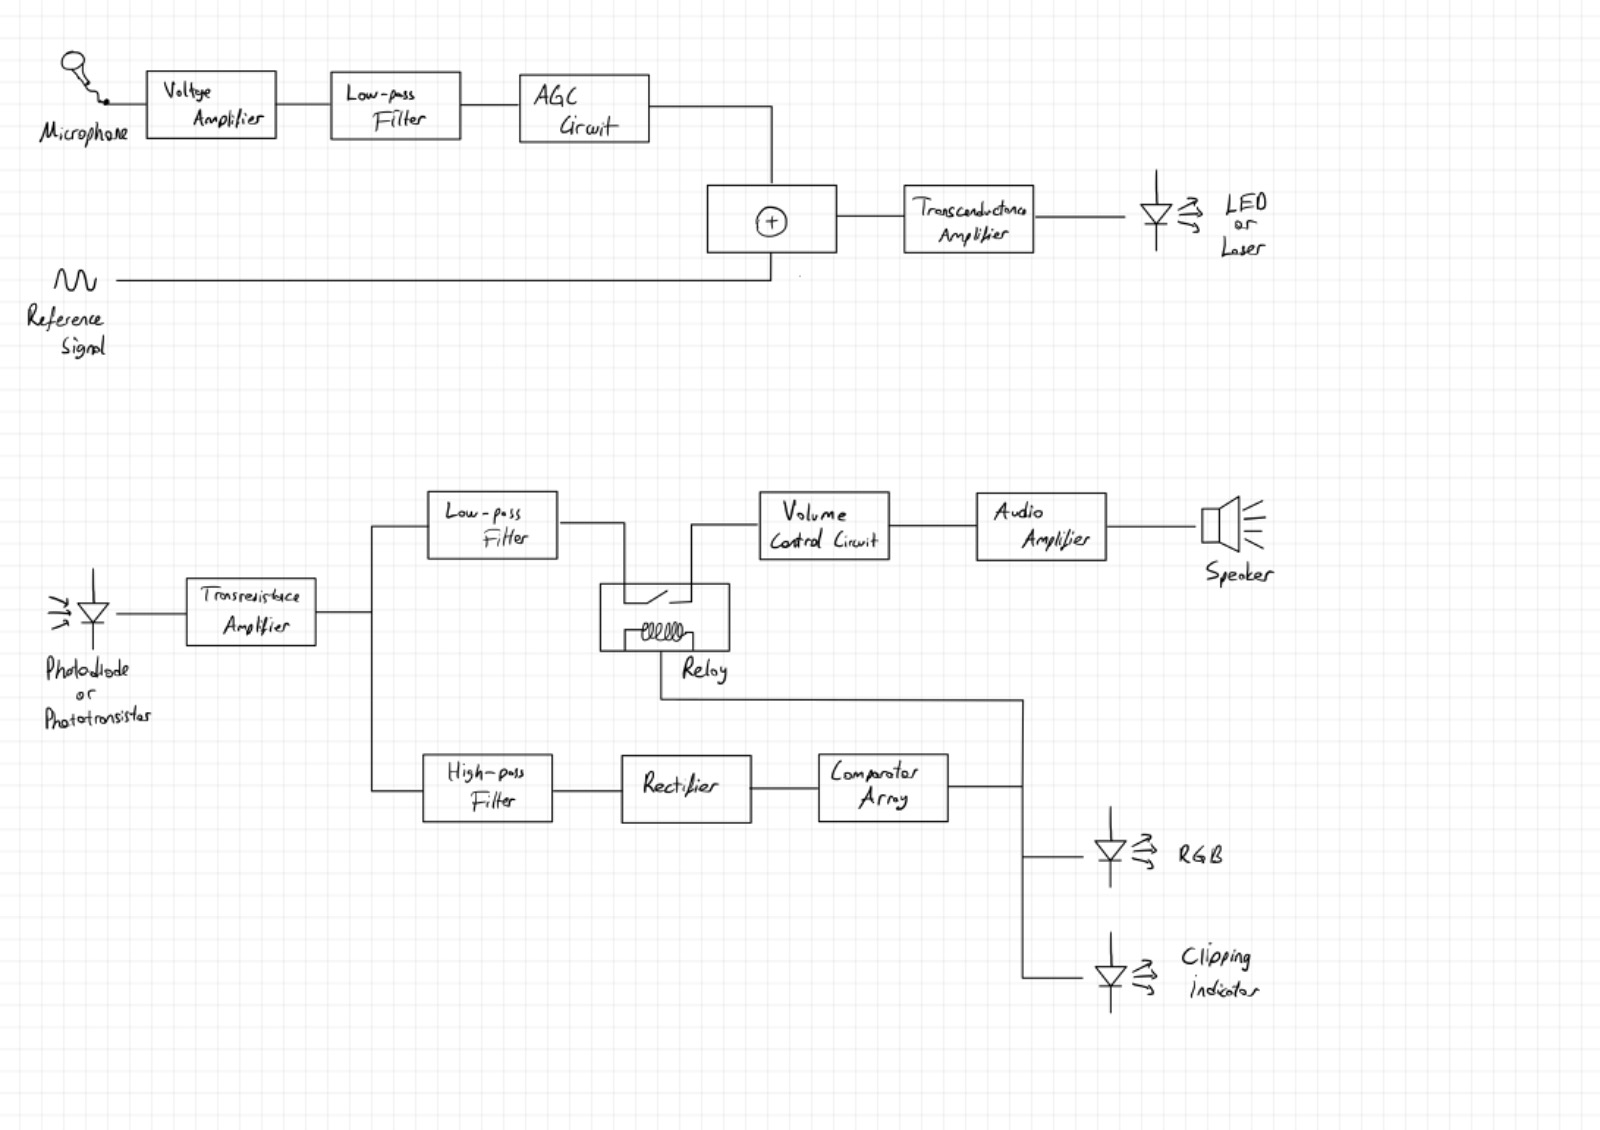
\includegraphics[width = 1\linewidth]{general_structure.jpeg}
    \caption{General Structure}
    \label{general}
\end{figure} 
\vspace{-0.8cm}
\section{Transmitter Side}
\vspace{-0.1cm}
\subsection{Input and Early Stage Amplification}
The microphone is basically a resistor; its resistance is dependent on the audio waves. To convert audio signals to electrical signals, a voltage divider topology can be used. Since the output signal of that conversion gives a very small signal, it is much more sensitive to any noise. Therefore, just after that stage, this small signal should be directly amplified by using a common source or common emitter amplifier. This pre-amplifier gave a less noise-sensitive and more operatable voltage range signal. After that, it is thought to be fed that signal to a low pass filter to filter out only the human voice for other stages. 
\vspace{-0.5cm}
\subsection{Automatic Gain Control}

The automatic gain control circuit is mainly designed around an opamp which has passive negative feedback composed of several resistances connected between the output and inverting input of the opamp. On the other hand, the positive feedback network will be constructed from a voltage amplifier and a transconductance amplifier. For high amplitude signals, the output of the opamp will also be high. That high-voltage signal will pass through the voltage amplifier and be converted to a DC-like voltage with the help of a load resistor and a capacitor. That DC voltage will drive the transconductance amplifier and change the current stolen from the non-inverting input of the opamp, which is also the input of the audio signal, according to the amplitude of the output signal. 
\vspace{-0.3cm}

\subsection{Light Transmitter}

The constant gain audio signal and the high-frequency reference signal should be summed before transmission. This summation process is thought to be applied by adopting a simple opamp summing amplifier.     
\begin{figure}[htbp!]
    \centering
    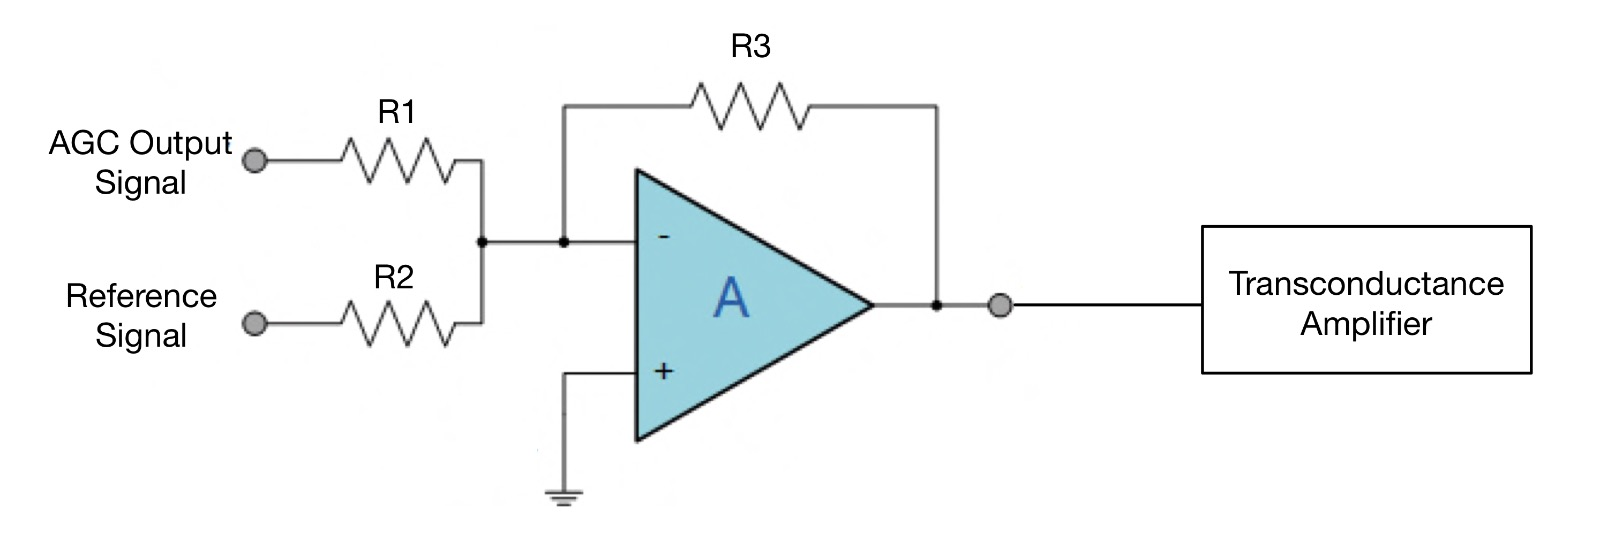
\includegraphics[width = 1\linewidth]{transconductance.jpeg}
    \caption{Summing connection scheme }
\end{figure} 
For transmission of the signal, the requirement of the light source can be supplied from a LED or a laser. Since the laser is more focused, any small misalignment of it can possibly result in an error for both calibrations and debugging processes. Since then, a LED has been decided to be used. For infrared LEDs also, an infrared-compatible receiver is needed, which is generally harder and more expensive to obtain. That is why a single-color visible light LED is determined to be used. In order to avoid any noise from environmental light sources, a plastic tube is thought to be included, which will be expandable to be able to observe the change of the signal strength by changing its length. 

The luminous intensities of LEDs are linearly dependent on the forward current passing through. That is why, after the summation of the audio and reference signal, a transconductance amplifier is needed. That way, the voltage signal input will be converted to a current output signal that will be fed through the LED transmitter.
\vspace{-0.45cm}
\section{Receiver Side}
\vspace{-0.1cm}
\subsection{Light Receiver}

On the receiver side, there is a need for some type of light detector to detect and receive the transmitted light which contains the audio signal. There are different types of photosensors, but two of the most appropriate of them are photodiodes or phototransistors. Each of those components has some pros and cons. To determine the most suitable one for the current application, some research has been conducted. We can see the characteristics and differences between them in Table \ref*{table1}. 

\begin{table}[htbp!]
    \begin{tabular}{|p{0.45\linewidth}|p{0.45\linewidth}|}
    \hline
    \textbf{Photodiode}                                                         & \textbf{Phototransistor}                                                                \\ \hline
    The photodiode is a semiconductor component that converts light energy into electrical energy. & Phototransistor is a semiconductor component that amplifies the current generated from light energy. \\ \hline
    It is composed of one PN junction diode.                                                   & It is composed of one NPN or PNP transistor that is sensitive to light.                                \\ \hline
    It can be used with a power supply, but it doesn't require it.                              & It requires a   power supply with proper biasing.                                                        \\ \hline
    It generates both voltage and current.                                                     & It only generates a current.                                                                             \\ \hline
    It is affordable.                                                                            & It is more expensive than a photodiode.                                                                  \\ \hline
    \end{tabular}
    \label{table1}
\end{table}


% \begin{figure}[htbp!]
%     \centering
%     \subfloat[\centering]{{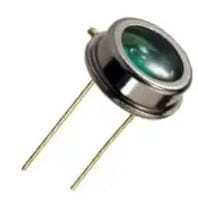
\includegraphics[height = 0.15\textwidth]{Photodiode.jpg} }}%
%     \quad
% \subfloat[\centering ]{{    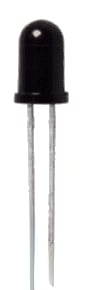
\includegraphics[height = 0.15\textwidth]{Phototransistor.jpg}}}%
%     \caption{Photodiode and Phototransistor}
%     \label{Photodiode}
% \end{figure} 


Since high-frequency signals are used in the project, in terms of the response time, the sensor should be quick, and also, as it is more affordable, a photodiode will be used. Depending on the project's progress and possible complications, this decision can be changed. 

Some further research is conducted for the implementation of it. There are two possible modes it can be used in terms of photovoltaic mode (Figure \ref{photovoltaic}) and photoconductive mode (Figure \ref{photoconductive}). In the photoconductive mode, since the photodiode is reverse biased, junction capacitance is small, which gives a fast switching feature to the sensor. As discussed earlier, since it gives a faster response photoconductive mode is planned to be implemented.

\begin{figure}[htbp!]
    \centering
    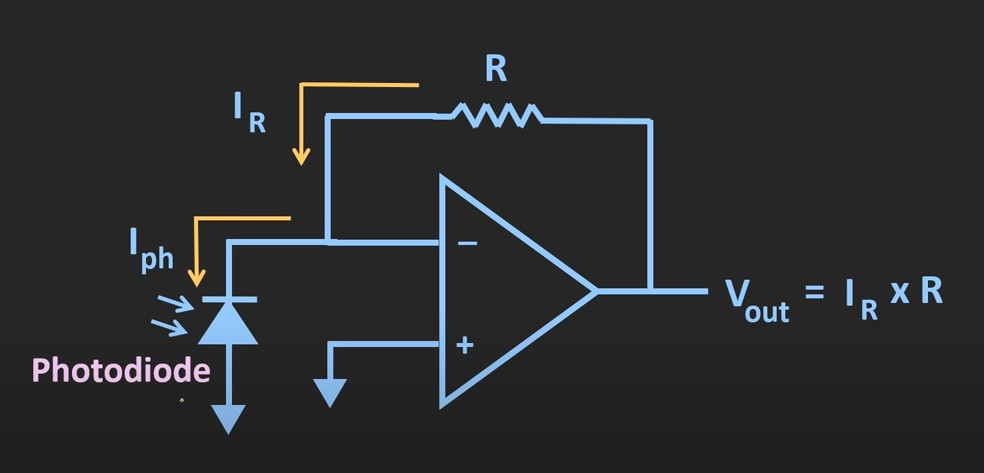
\includegraphics[width = 0.5\linewidth]{Photovoltaic.jpg}
    \caption{Photovoltaic mode}
    \label{photovoltaic}
    \end{figure} 

\begin{figure}[htbp!]
    \centering
    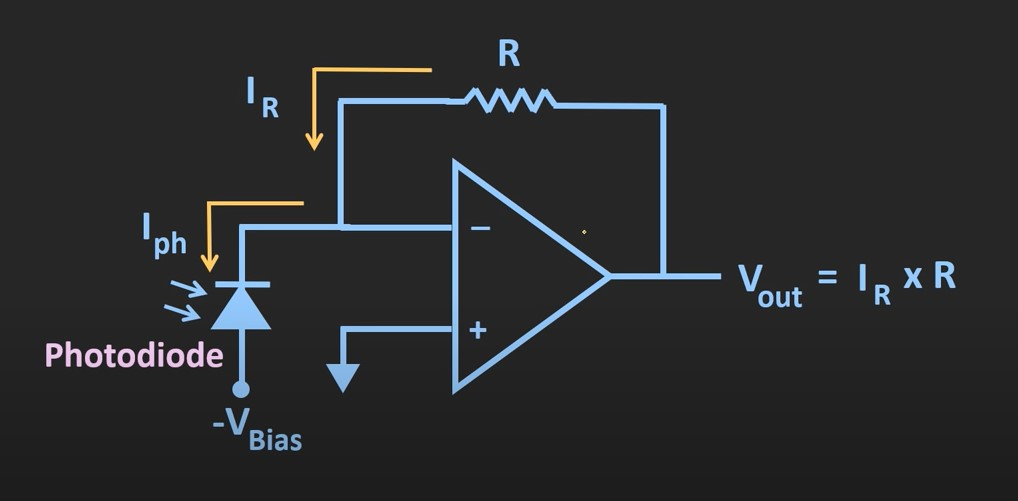
\includegraphics[width = 0.5\linewidth]{Photoconductive.jpg}
    \caption{Photoconductive mode}
    \label{photoconductive}
\end{figure} 
\vspace{-0.5cm}
\subsection{Demodulation and Speaker Side}
At the beginning of this stage, a simple opamp buffer will be planned to be used in order to prevent distortion while using the same signal as input for two stages in parallel. For the demodulation of the input signal (a.k.a. filtering out the high-frequency carrier components), a low-pass filter will be planned to be used. There are two basic options for low-pass filtering. The first one is passive RC/RL filters. They use few components but have no gain, and there is no tunability. The second one is active opamp-filters. Even though they seem more complicated, one can have more gain a more flexible design. The required low pass characteristic is given in Figure \ref*{low_pass_plot}
\begin{figure}[htbp!]
    \centering
    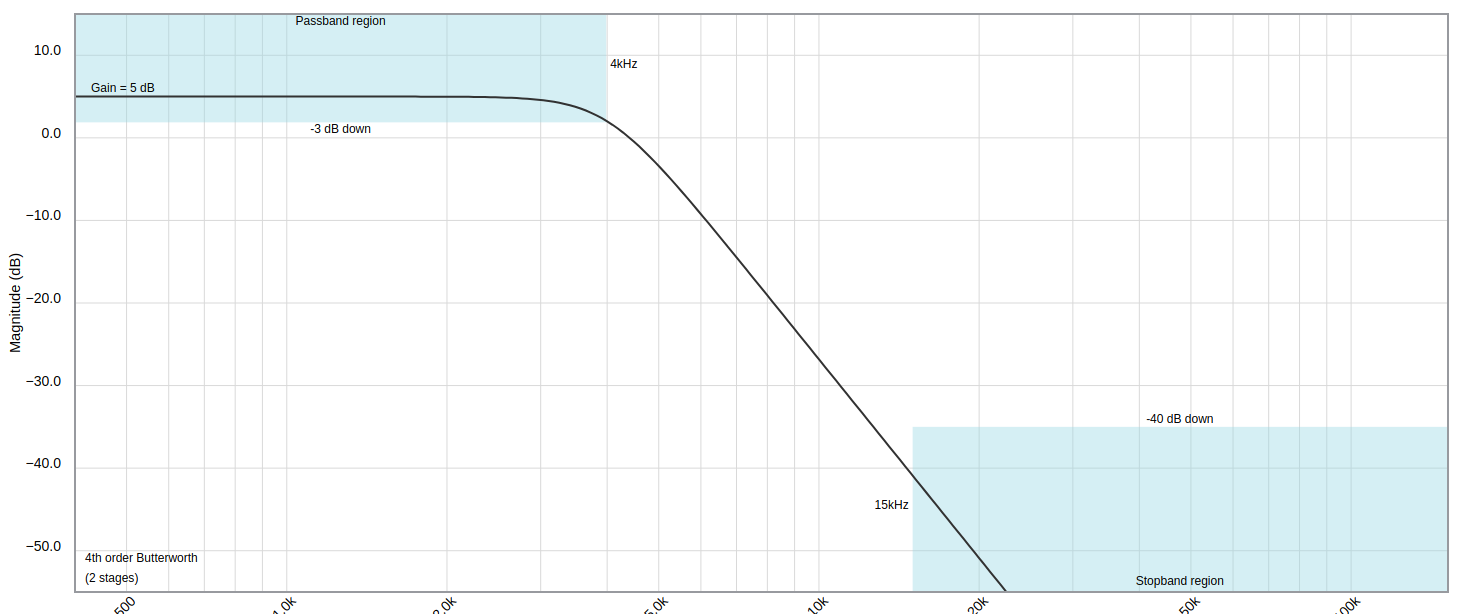
\includegraphics[width = 0.75\linewidth]{active_low_pass.png}
    \caption{Low pass filter frequency response}
    \label{low_pass_plot}    
\end{figure} 
Because of the aforementioned advantages, our design decision is to use an active two-stage low-pass filter with Butterworth response characteristics. A premature design is given in Figure \ref*{low_pass_sch}
\begin{figure}[htbp!]
    \centering
    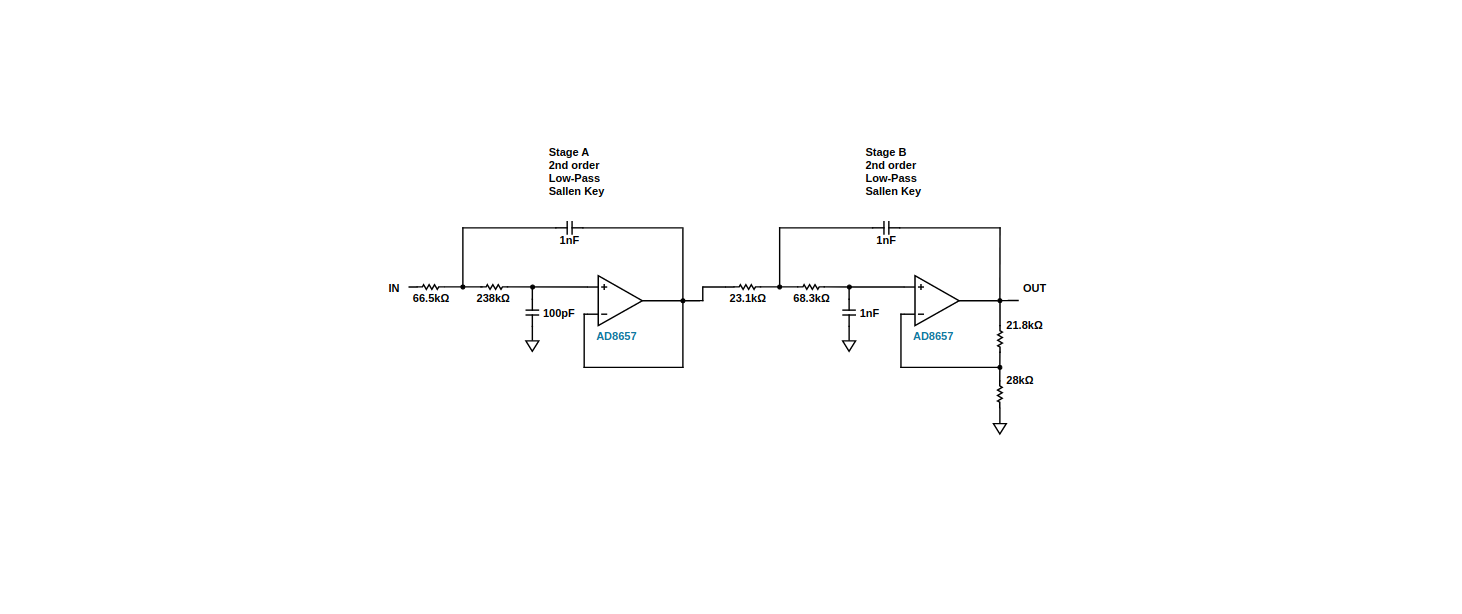
\includegraphics[width = 1\linewidth]{active_low_pass_circuit.png}
    \caption{Active low pass filter design}
    \label{low_pass_sch}    
\end{figure} 
\subsubsection{Low Signal Switch and Saturation Indicator}
The requirements of the projects indicate that if there is a small signal below a threshold, there should be no sound. On the other hand, it is given if there is a saturated signal, a LED should indicate this situation. So, to address both design problems, a design based on a voltage peak detector is proposed. The peak detector detects the peaks and the cascaded comparators compare the signal with reference dc values. To be able to adjust the threshold voltages, voltage dividers are utilized. For the low amplitude cut off, a MOSFET switch is added afterward. This stage of the design is given in Figure \ref*{saturated_ind} 
\begin{figure}[htbp!]
    \centering
    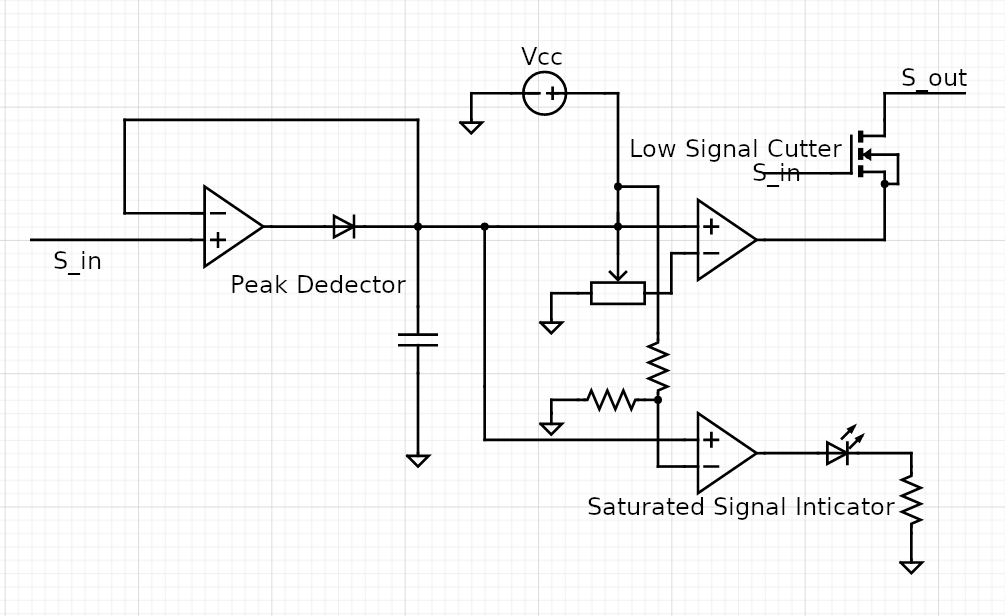
\includegraphics[width = 0.75\linewidth]{LowSignalSatSignal.png}
    \caption{Low and saturated signal switches.}
    \label{saturated_ind}    
\end{figure} 

\subsubsection{Volume Control}
In order to adjust the level of volume manually, a very well-known active volume control circuit called "Baxandall" will be used. The schematic of the block is given in Figure \ref*{Baxandall}. An opamp ic with two opamp such as TL072 or LM358, will be used as the amplifier in the schematic. 

\begin{figure}[htbp!] %https://www.ti.com/lit/ug/tidu034/tidu034.pdf?ts=1672401791602&ref_url=https%253A%252F%252Fwww.google.com%252F
    \centering
    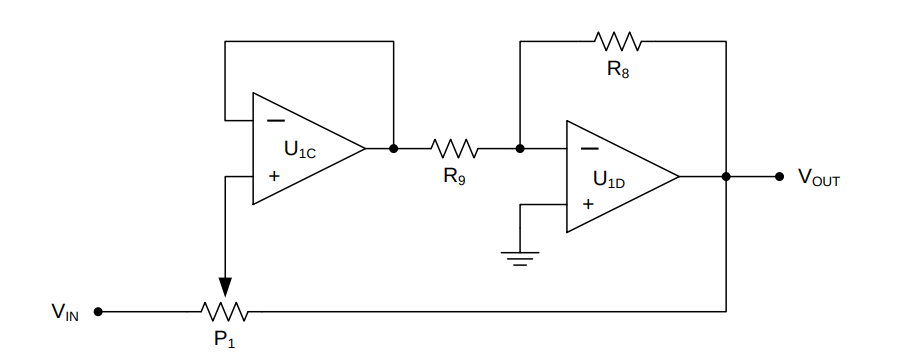
\includegraphics[width = 0.75\linewidth]{baxandall_volume_control.png}
    \caption{Active volume control circuit}
    \label{Baxandall}    
\end{figure} 
Since now we have a nice signal that carries the information needed, we should amplify it properly in order to drive the speaker. For the design purpose, we assume our speaker is 16\(\Omega\) , and our design constraint is that our speaker will operate with 1W power. There are a couple of options to drive speakers, such as Class A, Class B, Class AB, and Class C. For our driving purposes, a Class AB amplifier is planned to be used because of low distortion and higher efficiency compared to class A and B amplifier topologies. A schematic for such a stage is given in Figure \ref*{power_amp_sch}.
\begin{figure}[htbp!]
    \centering
    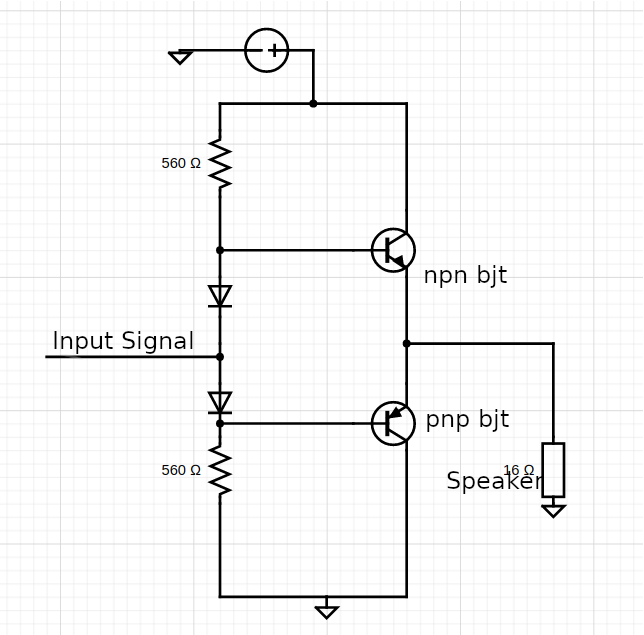
\includegraphics[height = 0.75\linewidth]{power_amp.png}
    \caption{Power amplifier and speaker unit.}
    \label{power_amp_sch}    
\end{figure} 
\vspace{-0.5cm}
\subsection{Signal Quality Indication}
One of the requirements of the project is an indication of the signal quality. To be able to extract the carrier signal from the overall signal, an active high-pass filter with a Chebyshev response. Similar to the low-pass case, a buffer stage will be added before the filter. The design with two stages is shown in Figure \ref*{active_high}.
\begin{figure}[htbp!]
    \centering
    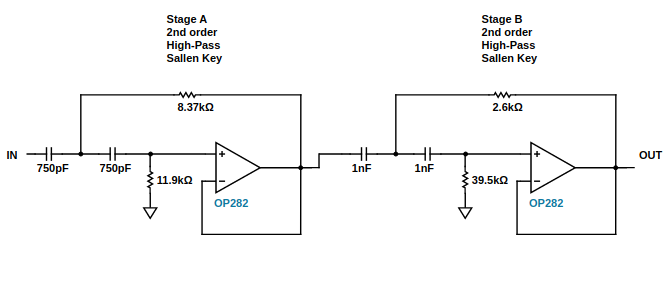
\includegraphics[width = 0.75\linewidth]{active_high_pass_circuit.png}
    \caption{Power amplifier and speaker unit.}
    \label{active_high}    
\end{figure} 

Again a simple peak detector will be utilized in order to discriminate the signal quality level. The peak value of the reference signal is then compared to four different reference voltages. Based on the comparison, an RGB light will display different colors depending on the voltage level. The specific colors that will be displayed are determined by the comparison of the voltage to the reference voltages, with green being displayed if the voltage is less than or greater than a certain range, red being displayed if the voltage is above a certain level, and blue being displayed if the voltage is above another level. The goal of this process is to display different colors of RGB light in different cases. The designed schematic is given in Figure \ref*{indicator}
\begin{figure}[htbp!]
    \centering
    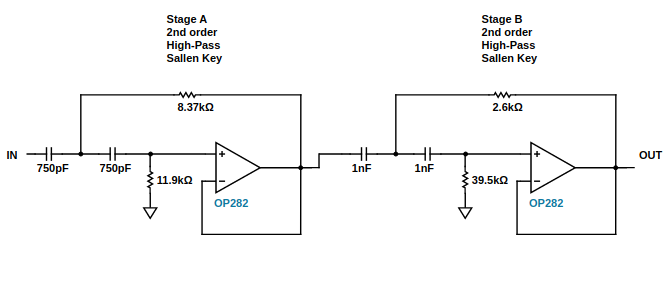
\includegraphics[width = 0.75\linewidth]{active_high_pass_circuit.png}
    \caption{Signal Level Indicator part}
    \label{indicator}    
\end{figure} 
\vspace{-0.4cm}
\section{Conclusion}
In this document, the proposal report of the term project of the EE313 course is presented. 

\end{document}

%%%%%%%%%%%%%%%%%%%%%%   EXAMPLE TABLE   %%%%%%%%%%%%%%%%%%%%%%%%%%%%%%%%
\begin{table}[H]
\begin{center}
    \caption{Resistance reading by color code convention.}
    \vspace{2mm}
    \begin{tabular}{||c | c | c||} 
        \hline
        Color Order & Value & Tolerance \\ [0.5ex] 
        \hline\hline
        Brown / Black / Red / Gold & 1k\( \Omega \) & \( \% \) 5  \\ 
        \hline
        Yellow / Violet / Red / Gold & 4.7k\( \Omega \) & \( \% \) 5   \\
        \hline
        Brown / Grey / Orange / Gold & 18k\( \Omega \) & \( \% \) 5  \\ [1ex] 
        \hline
    \end{tabular}
\end{center}
\end{table}


%%%%%%%%%%%%%%%%%%%%%%   EXAMPLE IMAGE   %%%%%%%%%%%%%%%%%%%%%%%%%%%%%%%%
\begin{figure}[H]
\centering
\includegraphics[width = 0.75\linewidth]{5.png}
\caption{Circuit schematic for the step 5}
\end{figure} 

%%%%%%%%%%%%%%%%%%%%%%   EXAMPLE IMAGE FROM PDF   %%%%%%%%%%%%%%%%%%%%%%%%%%%%%%%%
\begin{figure}[H] \centering{
    \includegraphics[scale=0.25]{2a_plot.pdf}}
    \caption{Experiment 2}
\end{figure}
%%%%%%%%%%%%%%%% Deneme Push